  \subsection{Correción del factor de potencia}
    \subsubsection{Cálculo del capacitor de compensación}
      
       Usando la ecuación~(\ref{eqn:CorrecFp}) se determina el valor del capacitor de compensación

      \begin{align*}
        %\varphi = sen ^{-1} \left( \dfrac{A}{B} \right) = sen ^{-1} \left( \dfrac{0,944\ V}{1,01\ V} \right) \hspace{20pt} \Longrightarrow \hspace{20pt} \Aboxed{\varphi = 69,17\ ^{\circ}}\ .
        C = \frac{25,22~W \cdot \tan(69,17~^{\circ} )}{(213~V)^2 \cdot 2 \cdot \pi \cdot 50~Hz }  \hspace{20pt} \therefore \hspace{20pt} \Aboxed{C = 4,65~[\mu F]}~.
      \end{align*}

        También es posible encontrar el valor del capacitor conociendo el factor de potencia, de acuerdo
        con el gráfico de la Figura~\ref{fig: Curva Cap_FDP}, que corresponde con un valor de capacitancia de $3,63~\mu F$. 

        \begin{figure}[H]
          \centering
            \frame{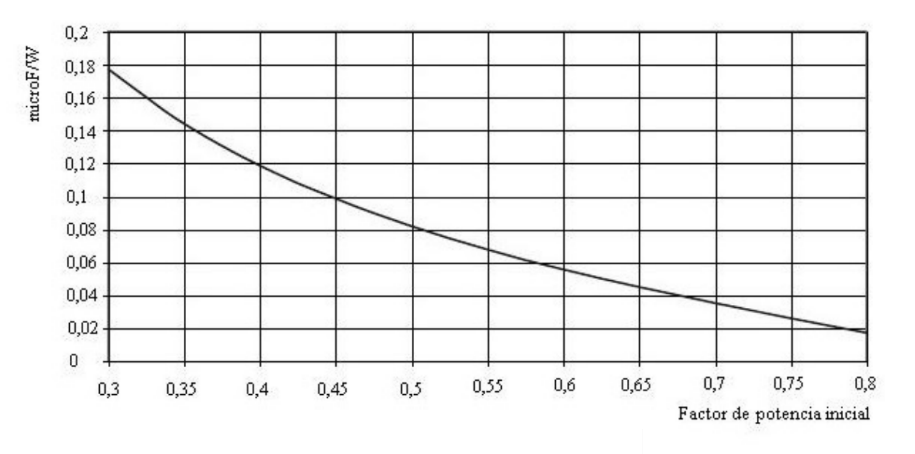
\includegraphics[width=0.7\textwidth]{Imagenes/ActividadPractica/CorreccionDeFdP/Curva Capa_FDP.png}}
            \caption{Curva Capacitancia-Factor de Potencia.}
            \label{fig: Curva Cap_FDP}
        \end{figure}

        

    \subsubsection{Medicion del factor de potencia corregido}

          Como se dificulta medir la diferencia de fase entre una señal y otra con el método del modo X-Y,
          se procede a determinar dicho desfasaje a partir de las señales en el dominio del tiempo. 
          Se dispone de un capacitor de valor 4,7[$\mu$F], con lo cual se cumple el requisito presentado
          anteriormente. Se procede a la conexión del mismo, y se observa en el osciloscopio el resultado.
        
        \begin{figure}[H]
          \centering
          \frame{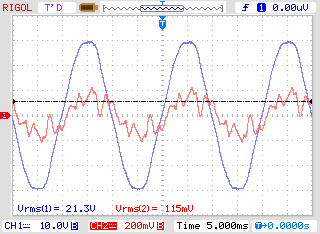
\includegraphics[width=0.7\textwidth]{Imagenes/ActividadPractica/CorreccionDeFdP/Exp2_11_Vin-Iin-ConCapacitor.png}}
          \caption{Señal resultante al agregar un capacitor.}
          \label{fig: Señal_Correccion}
        \end{figure}

        Se observa una importante cantidad de armónicos sumados a la señal de corriente, ésto debido
        a la deformación provocada por la carga conectada a la red.

         Con los nuevos valores de tension y corriente, se determina el valor de la nueva potencia 
         aparente

        \begin{align*}
          S = V_{rms}I_{rms}  \hspace{20pt} S=213\ [V]*0,115\ [A] \Longrightarrow \hspace{20pt} \Aboxed{S = 4,776 [VA]}.
        \end{align*}

          Adicionalmente, puede determinarse el factor de potencia corregido, a partir de las señales
          obtenidas en el tiempo. El principal problema es la cantidad de armónicos montados sobre 
          la señal de corriente, para resolverlo se debe aplicar un filtro pasa bajos a la misma, de
         ésta manera, es más sencillo realizar los cálculos.

        \begin{figure}[H]
          \centering
          \frame{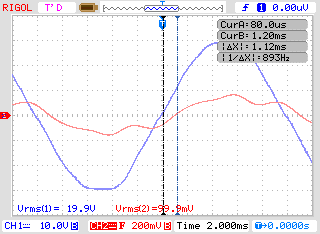
\includegraphics[width=0.7\textwidth]{Imagenes/ActividadPractica/CorreccionDeFdP/Exp2_15_Vin-Iin-ConCapacitorYFiltroEnOsc.png}}
          \caption{Medición del desfasaje de tensión y corriente.}
          \label{fig: Desfasaje tensión-corriente.}
        \end{figure}  

        Se tiene un semiperiódo de 10[ms] (lo que se corresponde con la frecuencia de la red de 50Hz),
        que equivalen a una pulsación de 180° , y usando la relación de tiempo/división del 
        osciloscopio junto con la relación entre ángulo y tiempo , se determina la correspondencia 
        en grados del desfasaje de la señal

        \begin{align*}
          \varphi = sen ^{-1} \left( \dfrac{t_{0}[ms] \cdot 180\ ^{\circ}}{0,5 \cdot T[ms]} \right) = sen ^{-1} \left( \dfrac{1,12[ms] \cdot 180\ ^{\circ}}{10[ms]} \right) \hspace{20pt} \Longrightarrow \hspace{20pt} \Aboxed{\varphi = 20,16\ ^{\circ}}\ .
        \end{align*}    

   